\chapter{Metodología}
\label{chap:metodologia}

 %De acuerdo a \cite{Barrett2009}, el modelo WCM...\\

\section{M\'etodo de Osweiler}
Es un m\'etodo que propone una manera de estimar los errores que se comenten en la utilizaci\'on de TLEs para la determinaci\'on de la posici\'on y la velocidad.
 El mismo consiste en utilizar un set de TLEs de un intervalo de dos semanas, y considerar el TLE m\'as pr\'oximo al tiempo de m\'aximo acercamiento (TLE  {\it{Primario}}) como el valor {\it{real}} o {\it{verdadero}}.\\
 A partir de esa premisa, propaga los TLEs anteriores hasta la \'epoca del TLE Primario y con las diferencias que resultan de la comparaci\'on, realiza los c\'alculos estad\'idticos de los valores medios y las varianzas, para construir la matriz Varianza Covarianza correpondiente al TLE Primario.\\
 Para hacer los estudios de validaci\'on de nuestra implementaci\'on del m\'etodo, de los 6 sat\'elites estudiados por Osweiler, dentro de 8 ventanas temporales distintas, nosotros hemos aplicado el m\'etodo a dos de ellos con caracter\'isticas similares a las misiones de CONAE y en particular a la misi\'on SAC-D, que hemos incorporamos como escenario propio de valiaci\'on ya que contamos con datos orbitales reales de mayor precisi\'on que los TLEs.

\section{Tratamiento sobre Datos de Misi\'on}
En esta etapa repetimos el m\'etodo que propone Osweiler considerando los datos de misi\'on generados por el CODS
como posici\'on verdadera.\\
La aplicaci\'on del m\'etodo implica:
\begin{itemize}
 \item Identificar el \'ultimo TLE del set: {\it{TLE primario.}}
 \item Extraer la \'epoca del TLE primario.
 \item Localizar el archivo CODS que contenga las efem\'erides que encierren la \'epoca del TLE primario.
 \item Interpolar las efem\'erides de CODS para generar una efem\'eride interpolada a la \'epoca del TLE primario.
 \item Propagar cada uno de los TLEs del set, hasta la \'epoca del TLE primario.
 \item Comparar los resultados de las propagaciones con los valores de la efem\'erides interpolada.
\end{itemize}

\begin{figure}[!h]
 \centering
 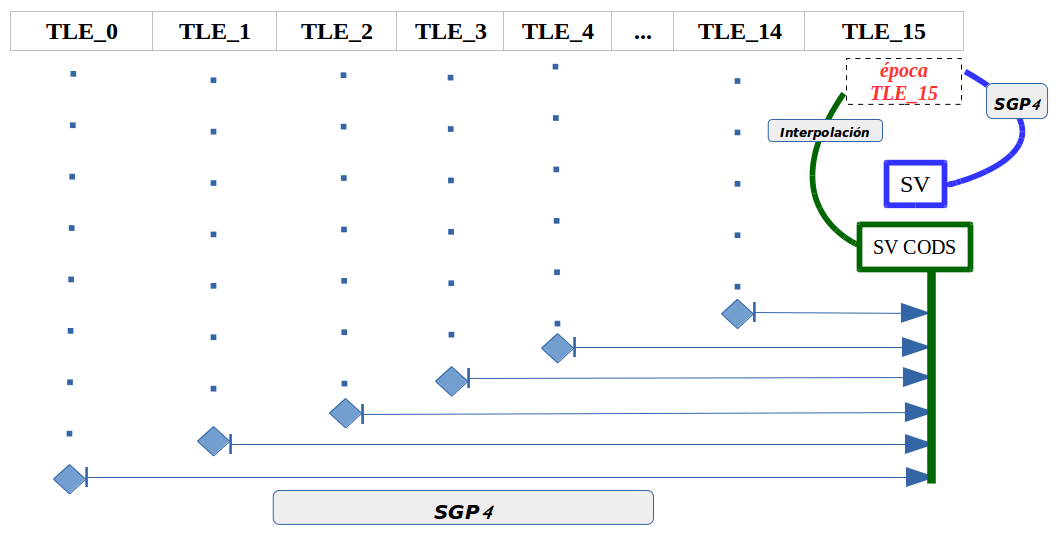
\includegraphics[width=0.7\textwidth]{imagenes/Osweiler_sobre_Cods.png}
 \caption{M\'etodo de Osweiler sobre datos CODS}
\end{figure}

\section{Preprocesamiento de los Datos de Misi\'on de CODS}
Para este trabajo CONAE nos facilit\'o el acceso a los datos orbitales de la misi\'on SAC-D.
Los datos se ecuentran montados en un servidor que contiene la informaci\'on organizada en archivos con formato ASCII, distribuidos en distintas carpetas seg\'un su clasificaci\'on.\\
Para la comparaci\'on que proponemos, solicitamos acceso a los archivos de efem\'erides orbitales ORBEPHEM, que ofrecen posiciones y velocidades tabuladas cada un minuto, en el Sistema de Referencia TOD (True of Date), en coordenadas cartesianas.

\subsection{ORBEPHEM}
Estos productos son generados luego de un post procesamiento que incluye una propagaci\'on ajustada por una determinaci\'on orbital. 
Cada archivo contiene un listado cronol\'ogicamente tabulado de posiciones y velocidades, dentro de un periodo de casi 3 d\'ias. ( doc\_interfaces)

La nomenclatura de los mismos respeta el siguiente formato:\\
\begin{verbatim}
 CODS_YYYYMMDD_HHMMSS_SACD_ORBEPHEM_TOD_XYZ_O.TXT
 
 Donde:
  CODS = Identifica el Servicio dentro del CUSS que presta la información.
  YYYYMMDD_HHMMSS = epoca de generación del dato.
  SACD = Identificación del Satélite.
  ORBEPHEM = Tipo de Dato, Efeméride Orbital (procesada a posteriori)
  TOD = Sistema de Referencia True of Date.
  XYZ = Tipo de efeméride, cartesiana.
  O = Operacional. 
\end{verbatim}


\subsection{Archivos Utilizados}
Si bien la nomenclatura de los archivos respeta una estructura, s\'olo se indica en el nombre, la fecha de generaci\'on de los datos y no puede desprenderse del mismo cu\'al es la \'epoca final e inicial de cada archivo, y no existe un registro del los gaps de datos ausentes. A su vez, las \'epocas contempladas en cada uno de ellos no está homogeneizada. Es decir, la fecha y hora inicial y final de cada registro es diferente para cada archivo.\\
Dada esta organizaci\'on, para el punto tres del procedimiento, referente a la localizaci\'on del archivo necesario para la comparaci\'on, la b\'usqueda se realiza de la siguiente manera:\\
Localizamos en primer lugar el archivo cuyo nombre coincide con la fecha de la \'epoca del TLE primario.
Como una misma fecha se encuentra en m\'as de un archivo, buscamos el archivo que contenga esa fecha y que adem\'as sea el m\'as actualizado de todos. Para ello, además del archivo cuyo nombre contiene la fecha del TLE primario, se enlistan los siguientes dos archivos y se ordenan en orden decreciente, de manera que el primer lugar de la lista lo ocupe el \'ultimo de los archivos seleccionados. Finalmente se comienza el proceso iterativo de abrir los archivos, evaluar el contenido y ver si se encuentran los dos registros que encierren la \'epoca del TLE.
Una vez que se encuentran las l\'ineas de efem\'erides que contienen la \'epoca de inter\'es se interpola, y se termina la iteraci\'on.

\noindent
Cantidad TOTAL de archivos $=  1454$\\
Cantidad media de resgistros por archivo $=  2688$\\
Archivo con el mayor n\'umero de registros $=  3042$\\
Archivo con el menor n\'umero de registros $=  142$\\

Im\'agenes comparativas entre los dos m\'etodos:\\

\begin{figure}[htbp]
 \centering
  \subfigure[Procesamiento de Datos de Mision]{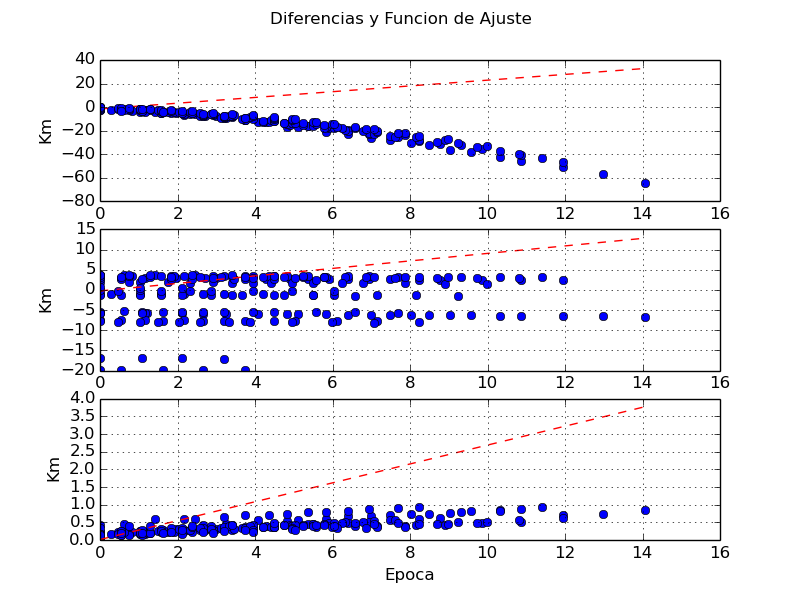
\includegraphics[width=0.46\linewidth]{imagenes/CODS_setCom_37673U_2}}
  \subfigure[Procesamiento de TLEs]{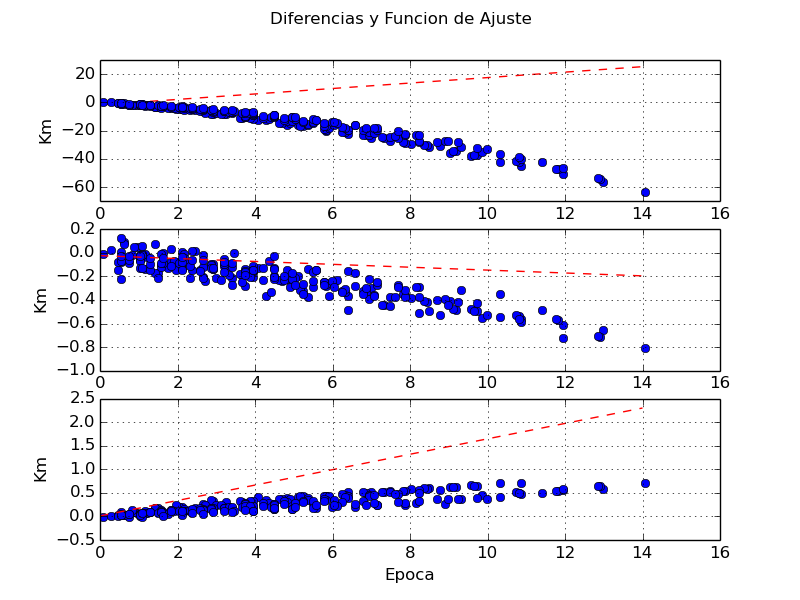
\includegraphics[width=0.46\linewidth]{imagenes/TLE_setCom_37673_2}}
 \caption{Resultado del m\'etodo de Pair-Wise Differencing considerando TLEs y Datos de Misi\'on.}
 \label{fig:test}
\end{figure}

\begin{verbatim}
------------------------------------------------------------------------
DIFERENCIAS: TLE-CODS
-------------------------------------------------------------------------
dv = -46.8489636874
dn = 2.35761559016
dc = 0.611728098324
\end{verbatim}

\begin{figure}[htbp]
 \centering
  \subfigure[Procesamiento de Datos de Mision]{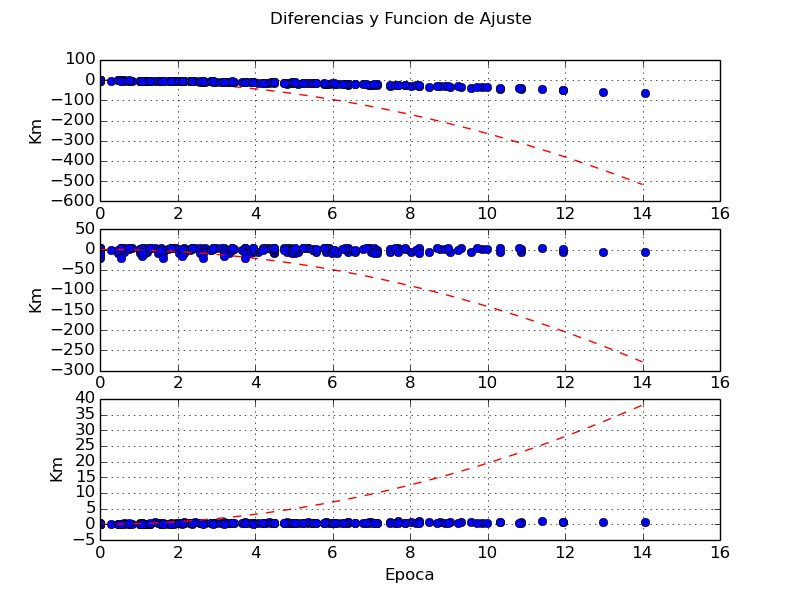
\includegraphics[width=0.46\linewidth]{imagenes/CODS_setCom_37673U_3}}
  \subfigure[Procesamiento de TLEs]{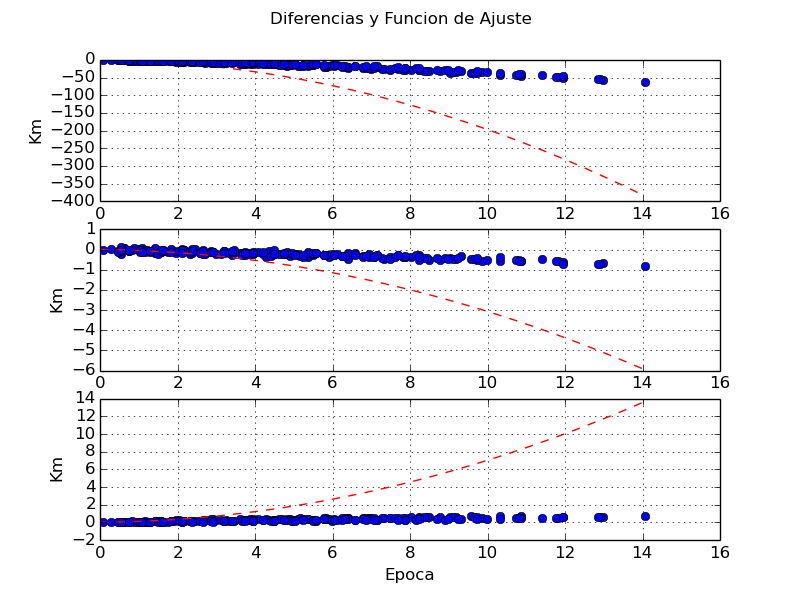
\includegraphics[width=0.46\linewidth]{imagenes/TLE_setCom_37673_3}}
 \caption{Resultado del m\'etodo de Pair-Wise Differencing considerando TLEs y Datos de Misi\'on.}
 \label{fig:test}
\end{figure}

\subsubsection{Ajuste Polyfit}

{\bf{numpy.polynomial.polynomial.polyfit}}

Returns:	

coef : ndarray, shape (deg + 1,) or (deg + 1, K)

    Polynomial coefficients ordered from low to high. If y was 2-D, the coefficients in column k of coef represent the polynomial fit to the data in y‘s k-th column.

residuals, rank, singular\_values, rcond : list

    These values are only returned if full = True

    resid – sum of squared residuals of the least squares fit rank – the numerical rank of the scaled Vandermonde matrix sv – singular values of the scaled Vandermonde matrix rcond – value of rcond.

    For more details, see linalg.lstsq.

\begin{verbatim}
Procesando datos TLE...
++++++++++++GRADO 2++++++++++++++++++
[array([-1.89669503, -0.73973919, -0.06103362])]
[[array([ 31434.82805686]), 3, array([ 1.68700379,  0.388,  0.056]), 5.1292e-14]]
++++++++++++GRADO 1++++++++++++++++++
[array([ 1.93247211, -1.78532883])]
[[array([ 31556.32886285]), 2, array([ 1.393,  0.24171176]), 5.1292e-14],]
\end{verbatim}

% \section{Graficos LAGEOS 8820}
% 
% \begin{figure}[H]
%  \centering
% \begin{subfigure}%{0.5\textwidth}
%   \centering
%   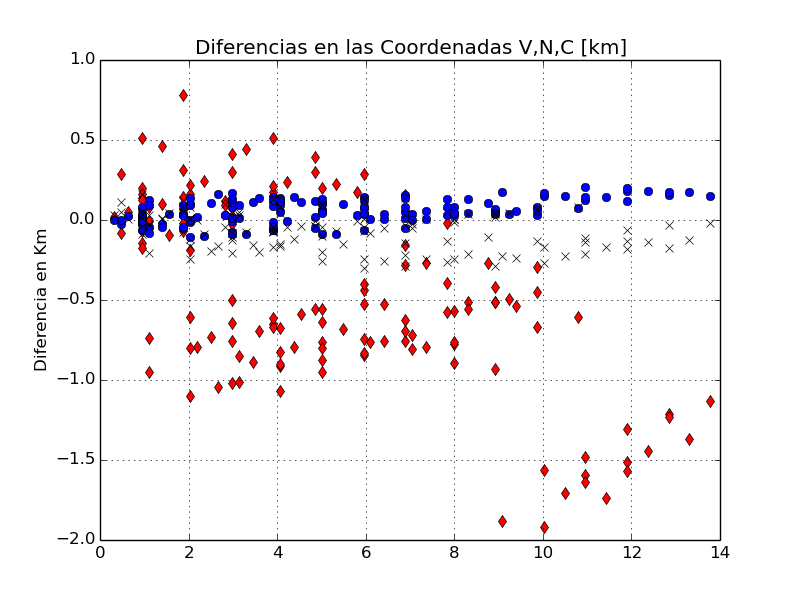
\includegraphics[width=0.7\linewidth]{imagenes/difTot8820.png}
%   \caption{A subfigure}
%   \label{fig:sub1}
% \end{subfigure}%
% \begin{subfigure}%{0.5\textwidth}
%   \centering
%   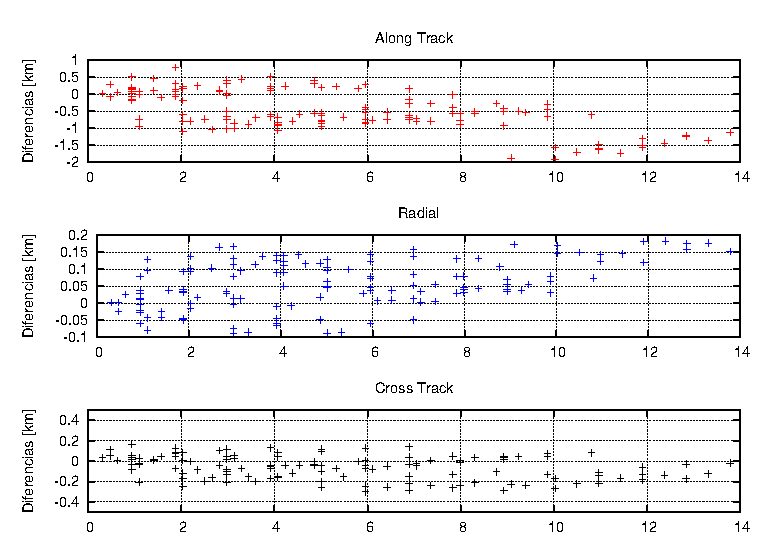
\includegraphics[width=0.7\linewidth]{imagenes/vncmultiplot}
%   \caption{A subfigure}
%   \label{fig:sub2}
% \end{subfigure}
% \caption{A figure with two subfigures}
% \label{fig:test}
% \end{figure}

\section{Transformaci\'on de Coordenadas}
[Montenbruck, Vallado Revisitin, Vallado Coorde Sys, tabla de Boado]

Para la comparaci\'on de las posiciones en coordenadas cartesianas, es necesario llevar ambos vectores a un mismo sistema de referencia.
La figura (ref) muestra un resumen de los distintos sistemas y las consideraciones de cada uno. 

\begin{figure}[!h]
  \centering
  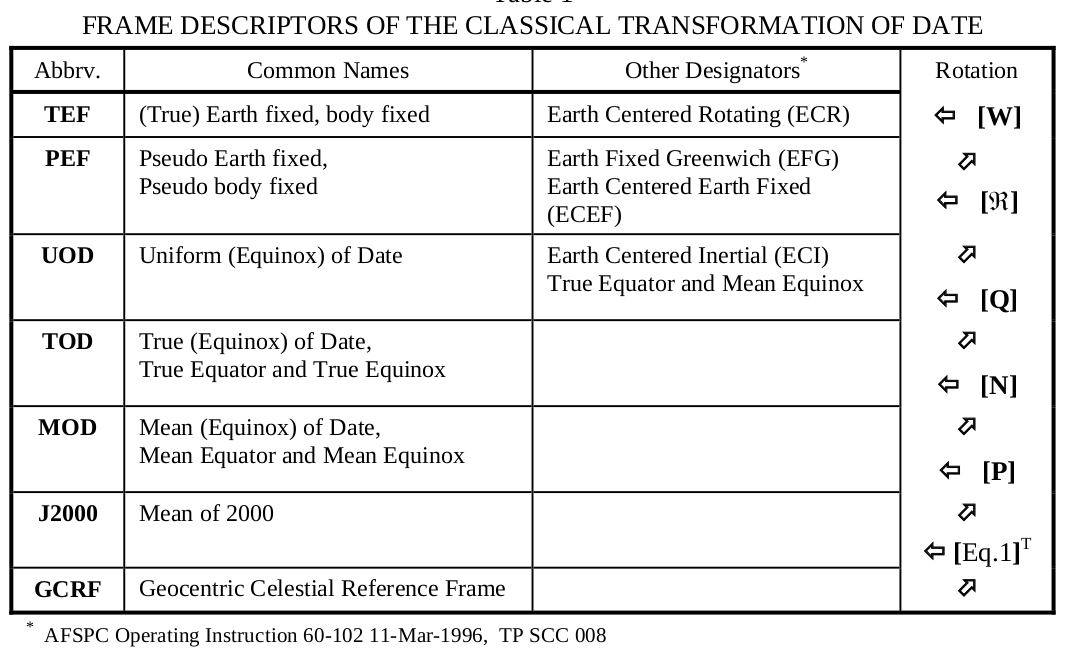
\includegraphics[width=0.7\textwidth]{imagenes/sistReferencias}
\end{figure}

En nuestro caso en particular, los datos que provee CODS se publican en el sistema TOD: True of Date (Verdadero de la \'epoca), mientras que los vectores de estado que genera el propagador SGP4 est\'an calculados en el sistema TEME: True Equator Mean Equinox (Ecuador Verdadero y Equinoccio Medio), tambi\'en denominado UOD (Uniform Equinox of Date).

Para la transformaci\'on de los datos de salida del SGP4 en el sistema TEME, al sistema TOD utilizamos la ecuaci\'on de los equinoccios, $EQ_{equinox}$, que nos permite transformar el equinoccio medio en el equinoccio verdadero.\\
Dado el vector de estado en el sistema TEME, $r_{_{TEME}}$, lo multiplicamos por la matriz de transformaci\'on en el eje z $Rot_{3}(EQ_{equinox})$ y obtenemos el vector de estado en el sistema TOD, $r_{_{TOD}}$.

\begin{equation}
 r_{_{TOD}} = [Q] r_{_{TEME}}
\end{equation}


 \[ Q =
\left( \begin{array}{ccc}
 cos(-EQ_{eqe}) & sin(-EQ_{eqe}) &  0 \\ 
 -sin(-EQ_{eqe}) & cos(-EQ_{eqe}) &  0 \\
 0 & 0 & 1
\end{array} \right) \] 


La ecuaci\'on de los equinoccios utiliza el modelo de nutaci\'on IAU-80 que considera los par\'ametros de nutaci\'on y los 106 coeficientes de Delaunay para el c\'alculo de la longitud $\Delta \Psi$ y la oblicuidad $\Delta \epsilon$.

\begin{equation}
 EQ_{eqe}=\Delta \Psi cos({\epsilon}) + 0.00264 \textquotedbl sin(\Omega_{(}) + 0.000063 \textquotedbl sin (2 \Omega_{(})
\end{equation}

Donde:

\begin{align*}
 \epsilon &= {\bar{\epsilon}} + \Delta \epsilon\\
 \Delta \Psi &= (A_{p} + A_{pl} tt) sin(a_{p_{i}})\\
 \Delta \epsilon &= (A_{e} + A_{el} tt) cos(a_{p_{i}})
\end{align*}

\begin{align*}
 tt &= (jd - 51544.5)/36525.0\\
 {\bar{\epsilon}} &= 84381.448 \textquotedbl - 46.8150 \textquotedbl tt - 0.00059 \textquotedbl tt^{2} + 0.001813 tt^{3}\\
 a_{p_{i}} &= a_{n1}M_{(}+a_{n2}M_{o}+a_{n3}\mu_{(}+a_{n4}D_{o}+a_{n5}\Omega_{(}
\end{align*}

Los coeficientes: $A_{p}$,$A_{pl}$,$A_{e}$,$A_{el}$,$A_{n_{i}}$ se extraen de la tabla de coeficientes de nutaci\'on de Seidelman(citar).

Y el resto de los par\'ametros se calcula seg\'un las expresiones:\\

\begin{align*}
 M_{(} & = M(tt)\\
 M_{o} & = M(tt)\\
 \mu_{(} &= \mu(tt)\\
 D_{o} &= D(tt)\\
 \Omega_{(} &= \Omega(tt)
\end{align*}

\section{Diferencias}
A partir de los datos de Misión. 

\begin{figure}[!h]
  \centering
  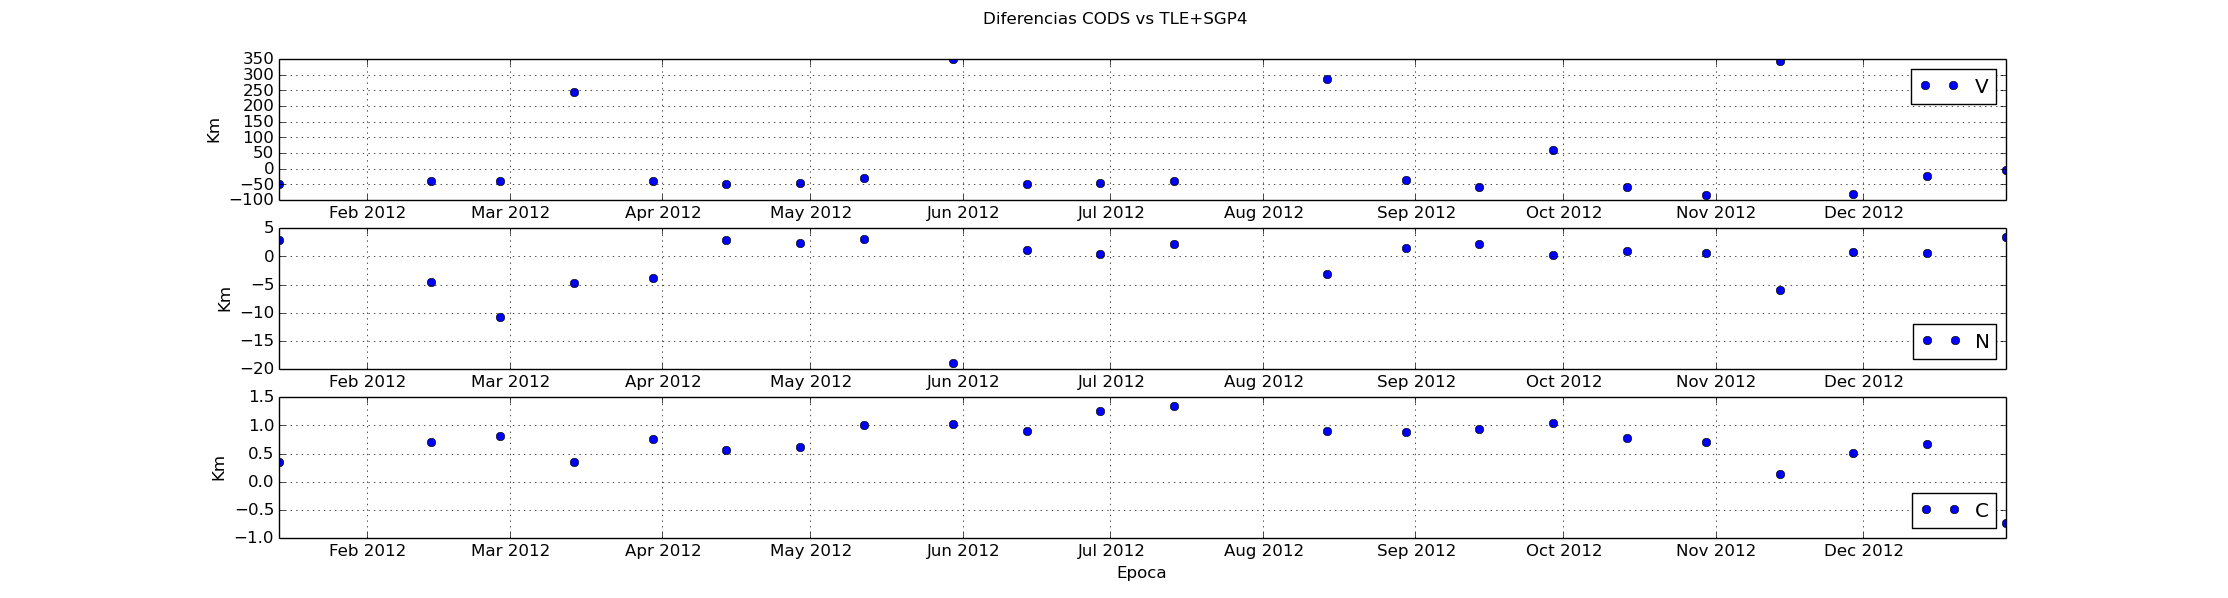
\includegraphics[width=\textwidth]{imagenes/sesgoTLE}
\end{figure}

\begin{itemize}
 \item Revisar escritura sobre datos CODS.
 \item Comparar defasaje inicial con defasaje de TLE respecto de GPS. (ver tendencias - empezar a diagramar los apédices)
 \item Comparar errores lineal vs cuadr\'atico.
\end{itemize}
